\documentclass[10pt]{amsart}
\usepackage[margin=1.4in]{geometry}
\usepackage{amssymb,amsmath,enumitem,url}
\usepackage{graphicx,subfig}
\usepackage{bm}
\graphicspath{ {./images/} }

\newcommand{\D}{\mathrm{d}}
\newcommand{\I}{\mathrm{i}}
\DeclareMathOperator{\E}{e}
\DeclareMathOperator{\OO}{O}
\DeclareMathOperator{\oo}{o}
\DeclareMathOperator{\erfc}{erfc}
\DeclareMathOperator{\real}{Re}
\DeclareMathOperator{\imag}{Im}
\usepackage{tikz}
\usepackage[framemethod=tikz]{mdframed}
\theoremstyle{nonumberplain}

\mdtheorem[innertopmargin=-5pt]{sol}{Solution}
%\newmdtheoremenv[innertopmargin=-5pt]{sol}{Solution}

\begin{document}
\pagestyle{empty}

\newcommand{\mline}{\vspace{.2in}\hrule\vspace{.2in}}

\noindent
\text{Hunter Lybbert} \\
\text{Student ID: 2426454} \\
\text{01-30-25} \\
\text{AMATH 502} \\
% header containing your name, student number, due date, course, and the homework number as a title.

\title{\bf {Homework 3} }


\maketitle
\noindent
Exercises come from a pdf provided by instructor.
\mline
\begin{enumerate}[label={\bf {\arabic*}:}]
\item For each of the following vector fields, find and classify all the fixed points, and
sketch the phase portrait on the circle. \\
\begin{enumerate}

\item $\dot \theta = 1 + 2 \cos \theta$ \\
\textit{Solution:} \\
We need to find where $\dot \theta = 0$.
Therefore we need 
\begin{align*}
1 + 2 \cos \theta &= 0 \\
\cos \theta &= -\frac 1 2.
\end{align*}
Which if we are assuming $\theta \in [0, 2 \pi)$ then we have fixed points at $\theta^* = \frac {2 \pi} 3, \frac {4 \pi} 3$.
See Figure \ref{fig:f1} for the phase portrait on the circle. \\
\qed \\

\item $\dot \theta = \sin \theta + \cos \theta$ \\
\textit{Solution:} \\
Once again we need to find where $\dot \theta = 0$.
Therefore we are looking for $\theta$ s.t.
\begin{align*}
\sin \theta + \cos \theta &= 0 \\
\cos \theta &= -\sin \theta.
\end{align*}
Assuming $\theta \in [0, 2 \pi)$ then this only holds for the following values of $\theta$ and thus we have fixed points at $\theta^* = \frac {3 \pi} 4, \frac {7 \pi} 4$.
See Figure \ref{fig:f1} for the phase portrait on the circle. \\
\qed \\

\item $\dot \theta = \sin 4 \theta$ \\
\textit{Solution:} \\
Once again we need to find where $\dot \theta = 0$.
Therefore we are looking for $\theta$ s.t.
\begin{align*}
\sin 4 \theta &= 0.
\end{align*}
Assuming $\theta \in [0, 2 \pi)$ then this only holds for the following values of $\theta$ and thus we have fixed points at $\theta^* = \frac {k \pi} 8$ for $k \in \{0, 1, 2, ..., 7\}$.
See Figure \ref{fig:f1} for the phase portrait on the circle. \\
\qed \\

\begin{figure}[h]
	\centering
	\includegraphics[height=.4\textwidth]{1_a_c.png}
 	\caption{We have sketched the phase portrait on the circle for problem 1a through 1c.}\label{fig:f1}
\end{figure}

\end{enumerate}

\newpage

\item There is a lot of context and build up to this problem in the assignment pdf which I will not transcribe here.
The important details will be included in their respective parts. \\

\begin{enumerate}

\item Graph the following function on the domain $-\pi \leq \phi < \pi$
\begin{align*}
f(\phi) = \begin{cases}
2\phi, & |\phi| \leq \frac \pi 2 \\
2 {\rm sgn}(\theta)\pi - 2\phi & |\phi| > \frac \pi 2.
\end{cases}
\end{align*}

\textit{Solution:} \\
See Figure \ref{fig:f2} for the graphs drawn by hand of the function $f(\phi)$. \\
\begin{figure}[h]
	\centering
	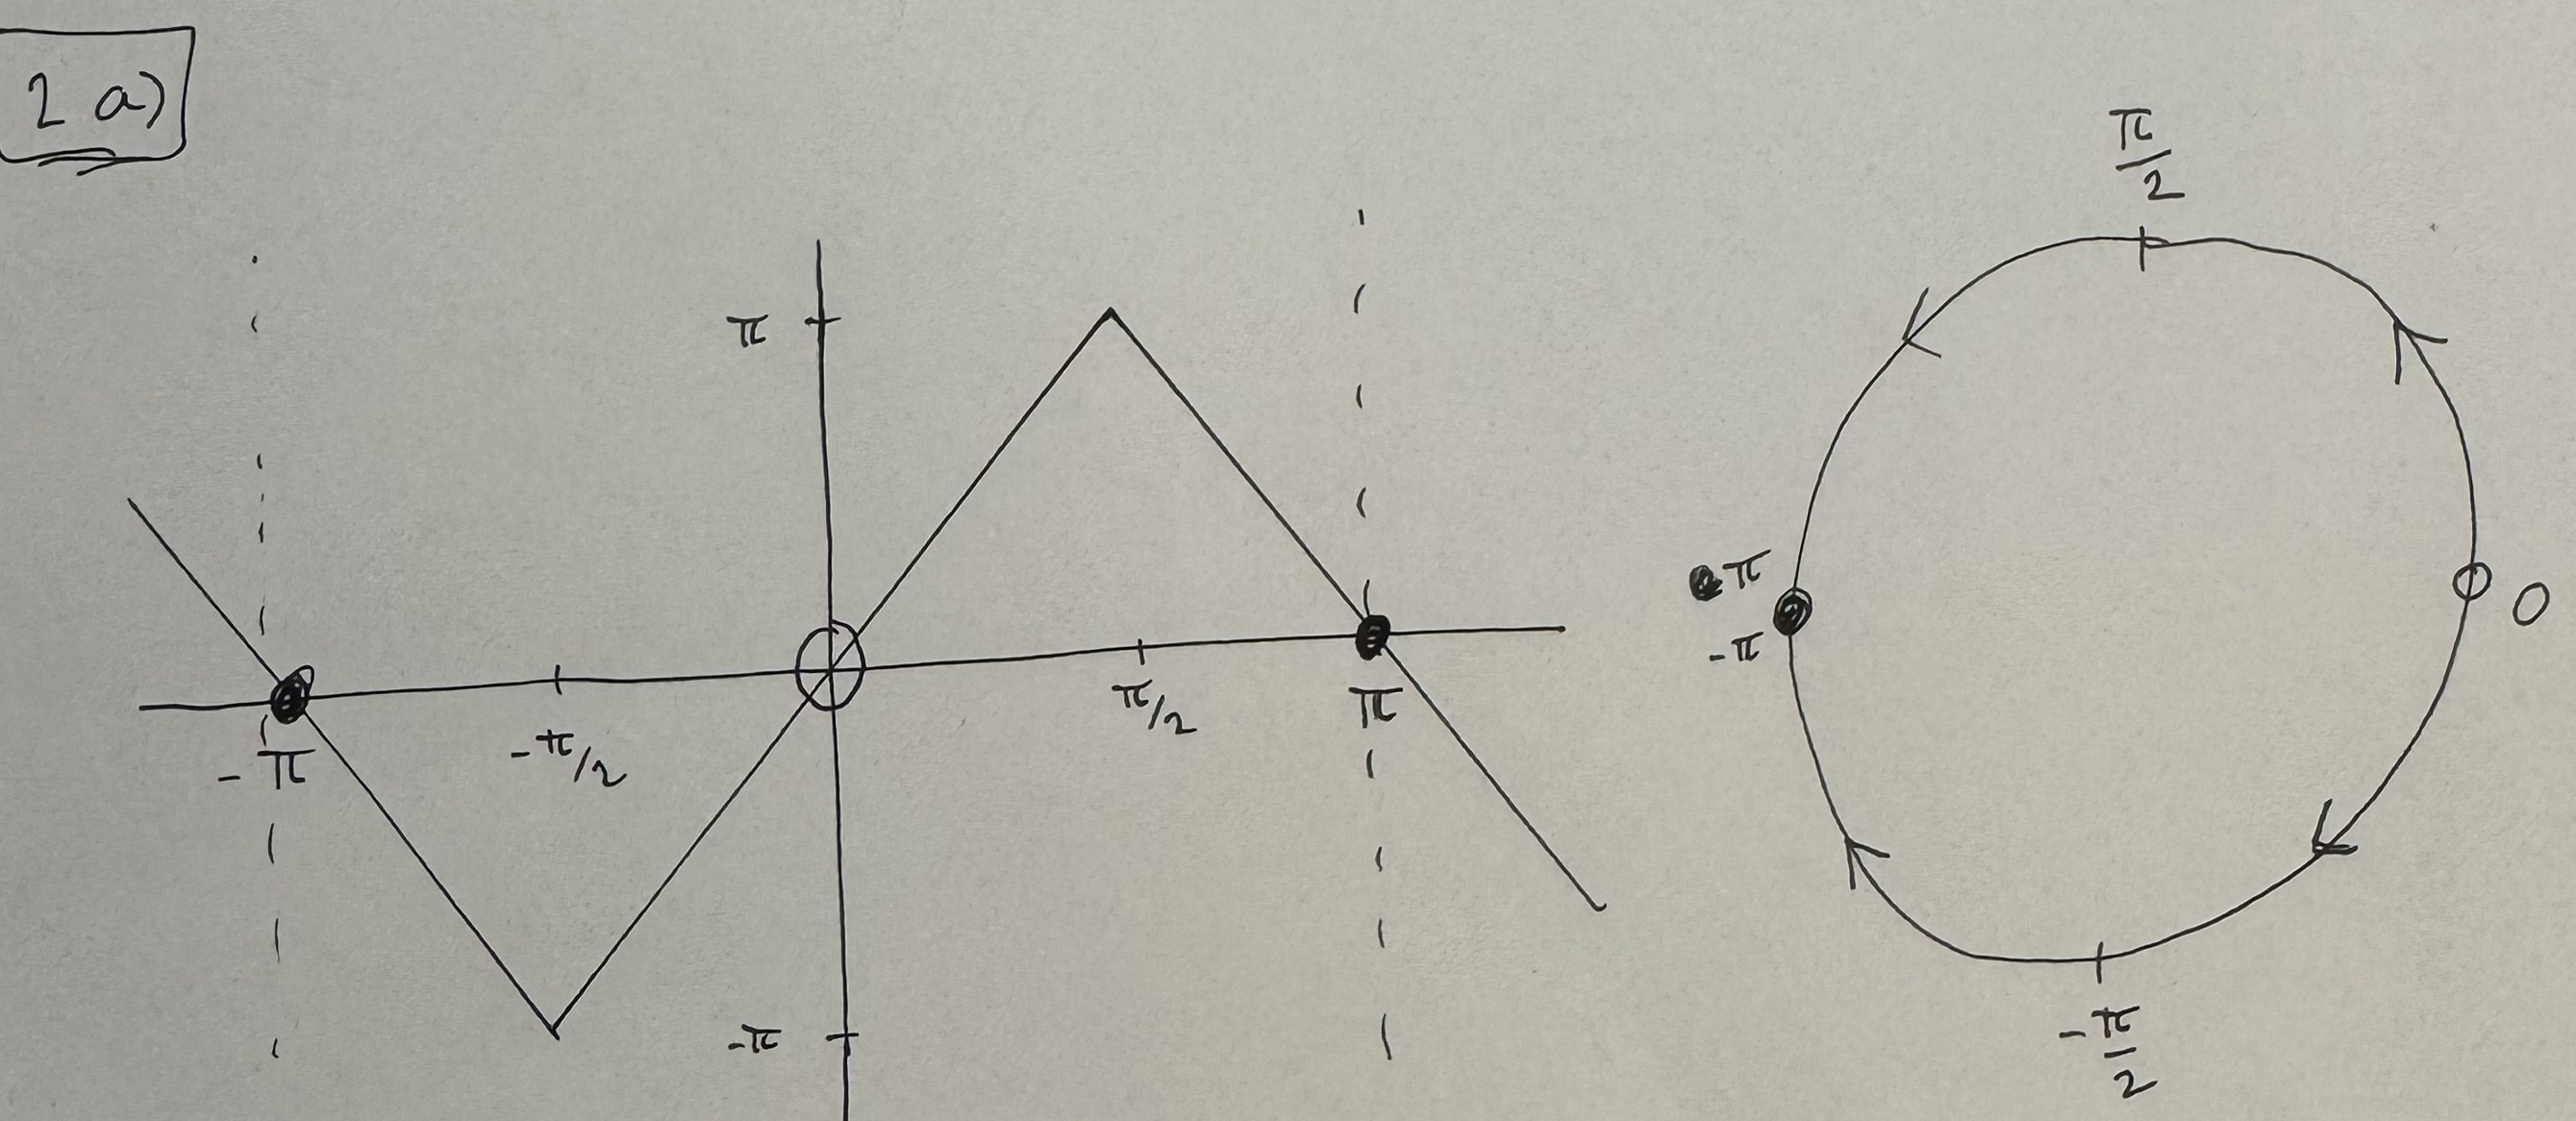
\includegraphics[height=.4\textwidth]{2_a.png}
 	\caption{We have sketched the function $f(\phi)$ as well as it's phase portrait on a circle.}\label{fig:f2}
\end{figure}

\qed \\

\item rite the dynamical system for the phase difference $\phi = \theta_s - \theta_f$ in terms of the dimensionless time $\tau = At$ and the dimensionless parameter $\mu = \frac {\Omega - \omega} A$. \\
\textit{Solution:} \\
We are also going to want to use the substitution $d \tau = A d t$.
Additionally, we are starting from the dynamical systems for $\theta_f$ and $\theta_s$ given by
$$\dot \theta_f = \omega + A f(\theta_s - \theta_f) \quad {\rm and }\quad \dot \theta_s = \Omega.$$
Let's start by manipulating these a bit
\begin{align}
\dot \theta_f &= \omega + A f(\theta_s - \theta_f) \nonumber \\
\frac {d \theta_f}{dt} &= \omega + A f(\theta_s - \theta_f) \nonumber \\
\frac {d \theta_f}{\frac 1 A d \tau} &= \omega + A f(\theta_s - \theta_f) \nonumber \\
A \frac {d \theta_f}{d \tau} &= \omega + A f(\theta_s - \theta_f) \nonumber \\
\frac {d \theta_f}{d \tau} &= \frac \omega A + f(\theta_s - \theta_f).
\label{eq:eq1}
\end{align}
Let's pause here, and manipulate this thing
\begin{align*}
\mu &= \frac {\Omega - \omega} A \\
\mu &= \frac \Omega A - \frac \omega A \\
\mu + \frac \omega A &= \frac \Omega A \\
\frac \omega A &= \frac \Omega A - \mu
\end{align*}
Now we can combine this result with equation \eqref{eq:eq1} as follows
\begin{align*}
\frac {d \theta_f}{d \tau} &= \frac \Omega A - \mu + f(\theta_s - \theta_f) \\
\frac {d \theta_f}{d \tau} &= \frac {\dot \theta_s} A - \mu + f(\theta_s - \theta_f) \\
\frac {d \theta_f}{d \tau} - \frac {d \theta_s} {A d t} &= - \mu + f(\theta_s - \theta_f) \\
\frac {d \theta_f}{d \tau} - \frac {d \theta_s} {d \tau} &= - \mu + f(\theta_s - \theta_f) \\
\frac {d \theta_f}{d \tau} - \frac {d \theta_s} {d \tau} &= - \mu + f(\theta_s - \theta_f) \\
\frac {d \theta_s} {d \tau} - \frac {d \theta_f}{d \tau} &= \mu - f(\theta_s - \theta_f) \\
\frac {d \theta_s - d \theta_f} {d \tau} &= \mu - f(\theta_s - \theta_f) \\
\frac {d \phi} {d \tau} &= \mu - f(\phi) \\
\end{align*}
We now have a the desired dynamical system. \\
\qed \\

\item Find the values of $\mu$ for which the firefly will be phase-locked to the stimulus. \\
\textit{Solution:} \\
\begin{align*}
\frac {d \phi} {d \tau} &= \mu - f(\phi) \\
0 &= \mu - f(\phi) \\
f(\phi) &= \mu
\end{align*}
Therefore whenever $\mu \in [-\pi, \pi]$ we have a fixed point. \\
\qed \\

\item Using the definition of $\mu$ and your answer from part (c), find the range of
frequencies of the stimulus $\Omega$ for which the firefly will be phase-locked to the
stimulus. \\
\textit{Solution:} \\
\begin{align*}
-\pi \leq \mu \leq \pi \\
-\pi \leq \frac {\Omega - \omega} A \leq \pi \\
-A\pi + \omega \leq \Omega \leq A\pi + \omega
\end{align*}
Therefore, $\Omega \in [-A\pi + \omega, A\pi + \omega]$. \\
\qed \\

\item What kind of bifurcation occurs at $\mu = \pm \pi$? Does this look like the usual
form for this type of bifurcation? If not, why not? \\
\textit{Solution:} \\
The bifurcation that occurs is a saddle node bifurcation, but it is not in the usual form.
For one, we typically see it as more of a sideways parabolic shape which we don't have here.
Secondly, we typically see the fixed points arise and continue to exist along their respective branches going off to infinity one way or the other.
However, this time we have the case where the two fixed points or branches arise and then eventually return to one another and finally disappearing again.
See Figure \ref{fig:f3} for further details on this odd saddle node bifurcation example. \\

\begin{figure}[h]
	\centering
	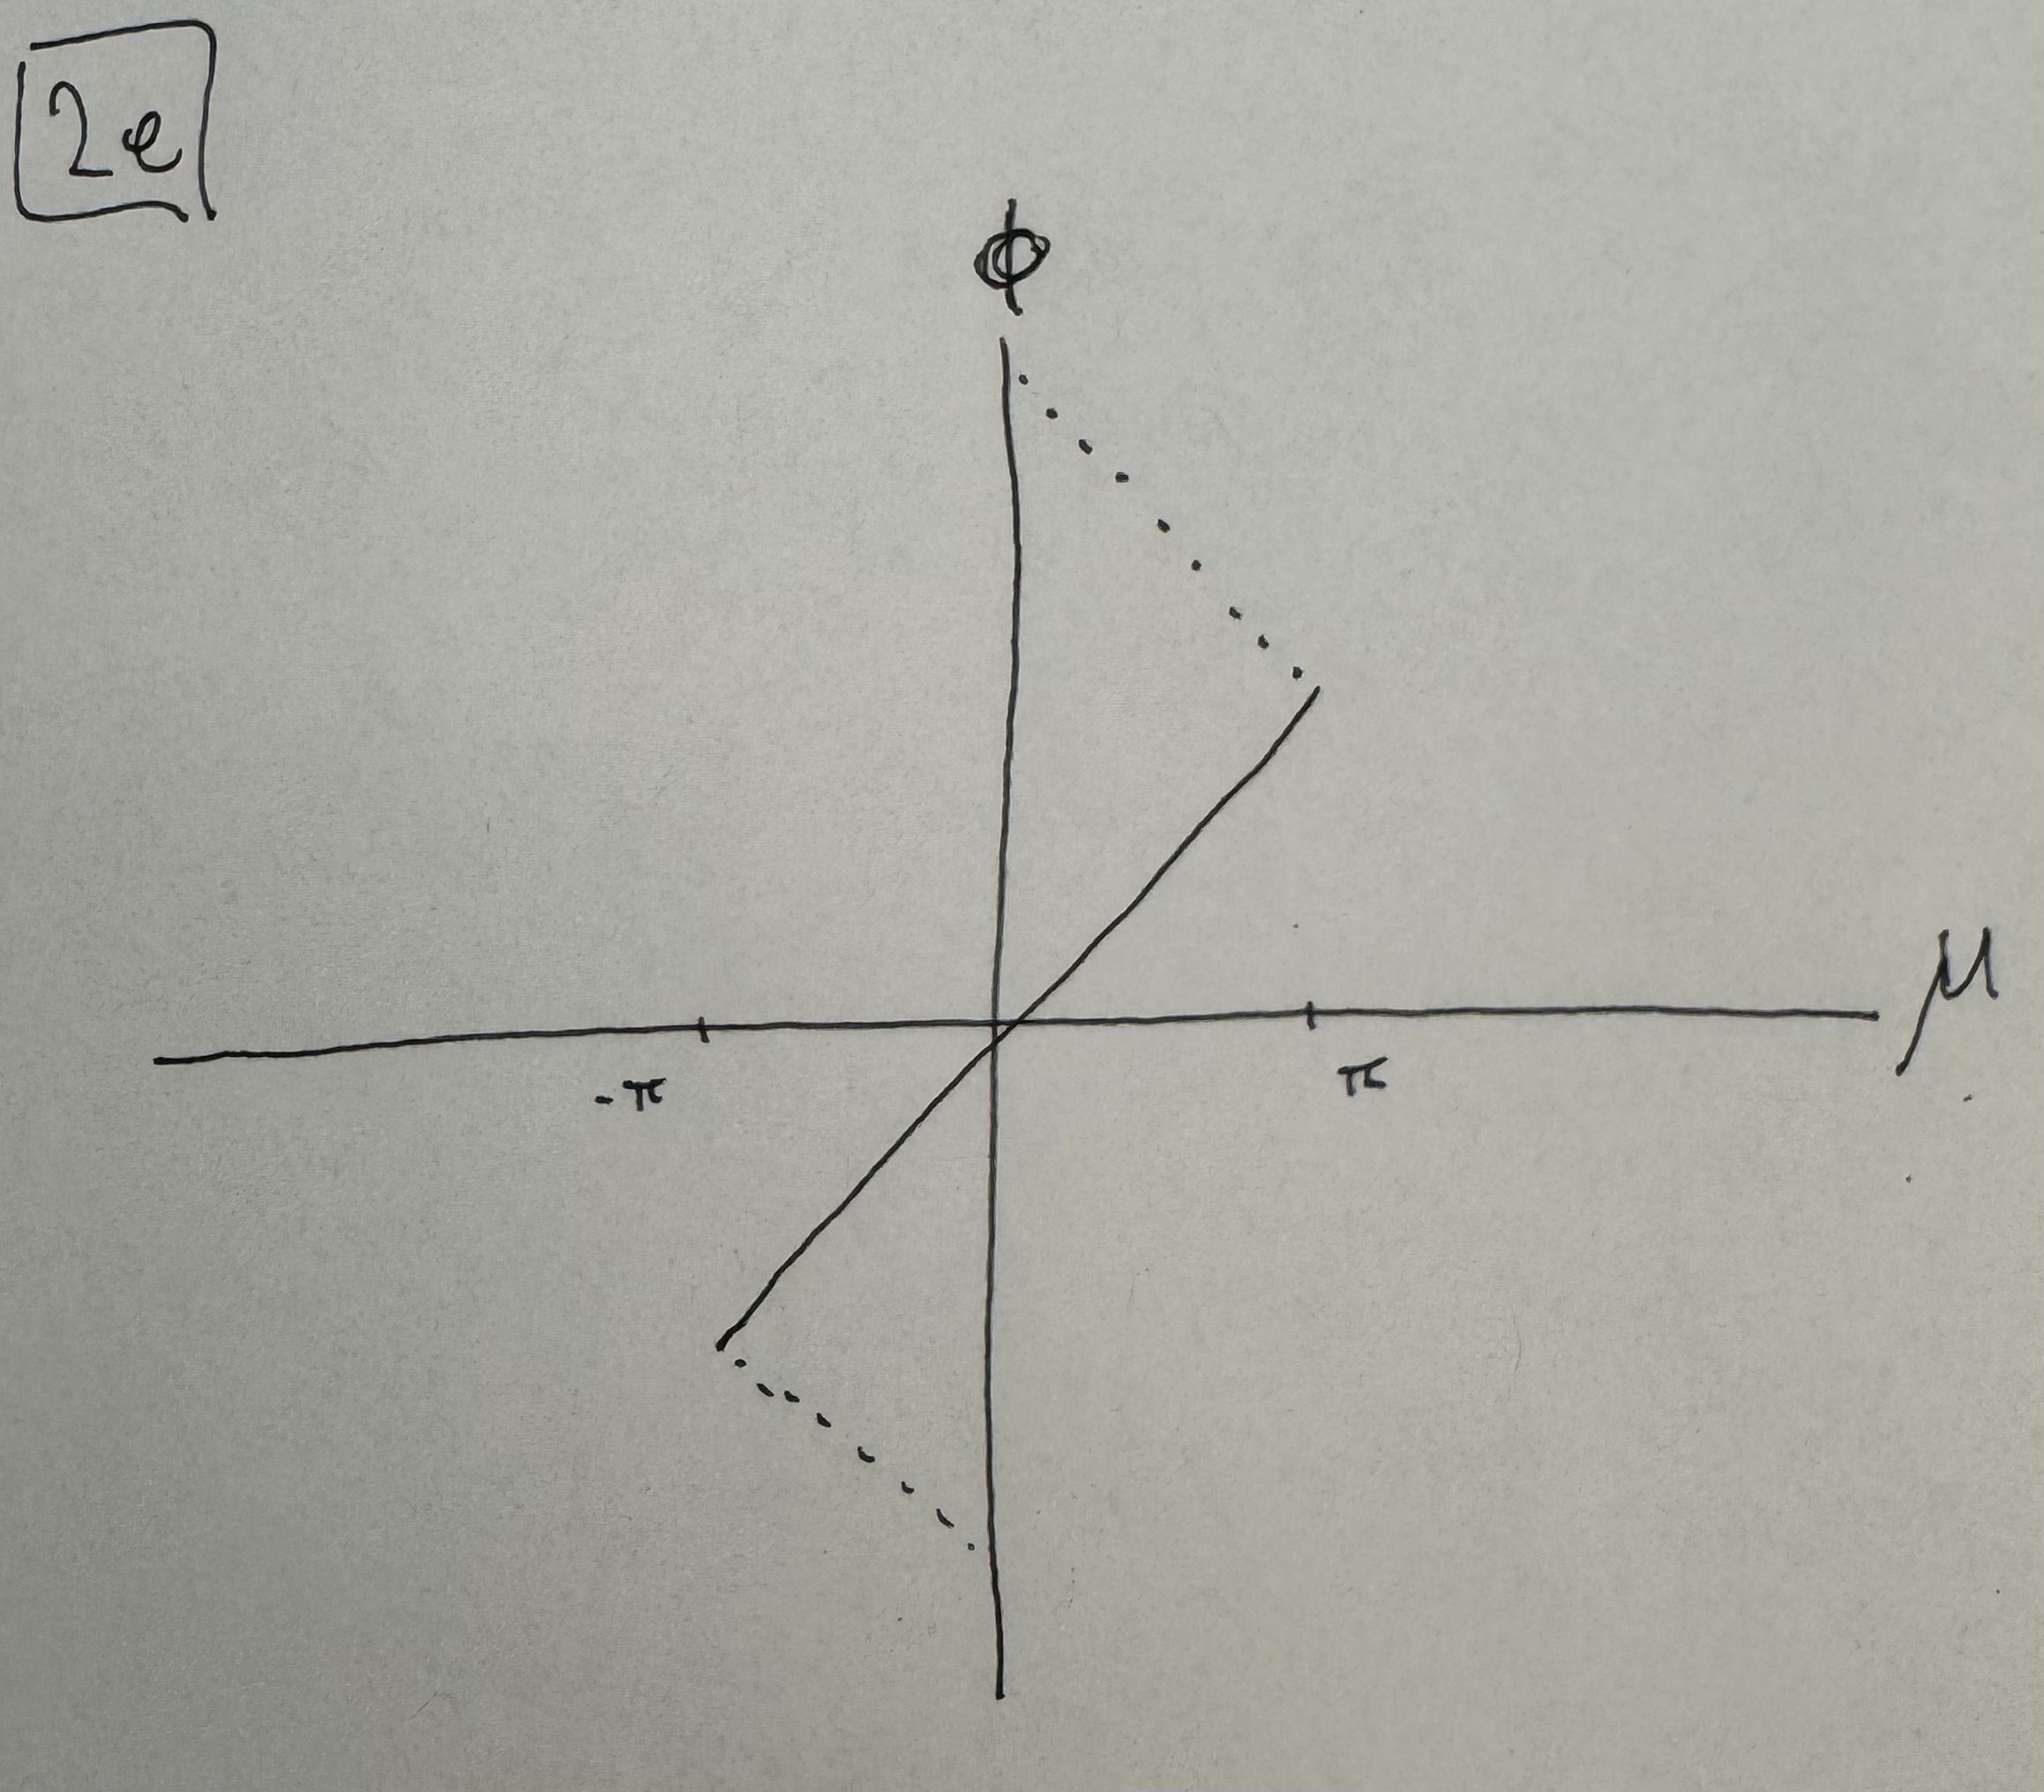
\includegraphics[height=.4\textwidth]{2_e.png}
 	\caption{The bifurcation diagram of $f(\phi)$ with respect to the parameter $\mu$.}\label{fig:f3}
\end{figure}

\item Assuming the firefly is phase-locked to the stimulus, find a formula for the
phase difference $\phi*$ (i.e. the stable fixed point). \\
\textit{Solution:} \\
When it is phase locked so we want $d\phi/d\tau = 0$ therefore we need $\mu - f(\phi^*) = 0$.
The first case to consider is if $|\phi^*| \leq \pi/2$ then we have
\begin{align*}
\mu - f(\phi^*) &= 0 \\
\mu &= f(\phi^*) \\
\mu &= 2\phi^* \\
\mu/2 &= \phi^*.
\end{align*}
The other case is slightly more complicated which is when $|\phi^*| > \pi/2$
\begin{align*}
\mu - f(\phi^*) &= 0 \\
\mu &= f(\phi^*) \\
\mu &= 2{\rm sign}(\phi^*)\pi - 2\phi^*.
\end{align*}
Again let's go with two more subcases where ${\rm sign}(\phi^*) = -1$ and ${\rm sign}(\phi^*) = 1$.
Starting with the negative case
\begin{align*}
\mu &= 2{\rm sign}(\phi^*)\pi - 2\phi^* \\
\mu &= 2\pi - 2\phi^* \\
- \mu/2 + \pi &= \phi^*.
\end{align*}
Now the positive case
\begin{align*}
\mu &= 2{\rm sign}(\phi^*)\pi - 2\phi^* \\
\mu &= - 2\pi - 2\phi^* \\
-\mu/2 - \pi &= \phi^*.
\end{align*}

\qed \\

\end{enumerate}

\newpage

\item Plot the phase portrait and classify the fixed point of the following linear systems. 
put the system in matrix form. \\

\begin{enumerate}

\item $\dot x = y, \quad \dot y = -2x - 3y$ \\
\textit{Solution:} \\
We can put this in the form of a 2 dimensional first order system as follows
\begin{align*}
\begin{bmatrix}
x \\ y
\end{bmatrix}^\prime
&= \begin{bmatrix}
0 & 1 \\
-2 & -3
\end{bmatrix} \begin{bmatrix}
x \\ y
\end{bmatrix}.
\end{align*}
Let's begin by finding the fixed points.
For a fixed point we need $y = 0$ and $-2x -3y = 0$.
Therefore we need $-2x = 0$ which implies the fixed point is when $(x^*,y^*) = (0, 0)$.
Furthermore, let's compute the eigenvalues of this system
\begin{align*}
\begin{bmatrix} 0 & 1 \\ -2 & -3 \end{bmatrix}
\begin{bmatrix} x \\ y \end{bmatrix}
	&= \lambda \begin{bmatrix} x \\ y \end{bmatrix} \\
\begin{bmatrix} 0 & 1 \\ -2 & -3 \end{bmatrix}
\begin{bmatrix} x \\ y \end{bmatrix} - \lambda \begin{bmatrix} x \\ y \end{bmatrix}
	&= \bm { 0 } \\
\left( \begin{bmatrix} 0 & 1 \\ -2 & -3 \end{bmatrix}
 - \lambda I \right)\begin{bmatrix} x \\ y \end{bmatrix}
	&= \bm { 0 } \\
\begin{bmatrix} -\lambda & 1 \\ -2 & -3 - \lambda \end{bmatrix}
\begin{bmatrix} x \\ y \end{bmatrix}
	&= \bm { 0 } \\
\end{align*}
This implies that we need
\begin{align*}
\det{ \left( \begin{bmatrix} -\lambda & 1 \\ -2 & -3 - \lambda \end{bmatrix} \right)} &= 0 \\
-\lambda(-3 -\lambda) + 2 &= 0 \\
\lambda^2 + 3\lambda + 2 &= 0.
\end{align*}
Thus we have
\begin{align*}
\lambda &= \frac{-3 \pm \sqrt{9 - 4(2)}} 2 \\
	&= \frac{-3 \pm 1} 2 \\
	&= -1, -2.
\end{align*}
Now we can calculate the eigenvectors!
First for $\lambda = -1$
\begin{align*}
\begin{bmatrix} 1 & 1 \\ -2 & -2 \end{bmatrix}
\begin{bmatrix} x \\ y \end{bmatrix}
	&= \bm { 0 }.
\end{align*}
This gives us $x + y = 0$ and $-2x -2y = 0$ therefore $x = -y$ and $y = y$ thus the eigenvector is
\begin{align*}
\begin{bmatrix} -1 \\ 1 \end{bmatrix}.
\end{align*}
Now for $\lambda = -2$ we have
\begin{align*}
\begin{bmatrix} 2 & 1 \\ -2 & -1 \end{bmatrix}
\begin{bmatrix} x \\ y \end{bmatrix}
	&= \bm { 0 }.
\end{align*}
This gives us $2x + y = 0$ and $-2x -y = 0$.
Therefore, $y = -2x$ and $x = x$ then the eigenvector is
\begin{align*}
\begin{bmatrix} 1 \\ -2 \end{bmatrix}.
\end{align*}
Now we can draw the qualitative phase portrait, see Figure \ref{fig:f4}

\begin{figure}[h]
	\centering
	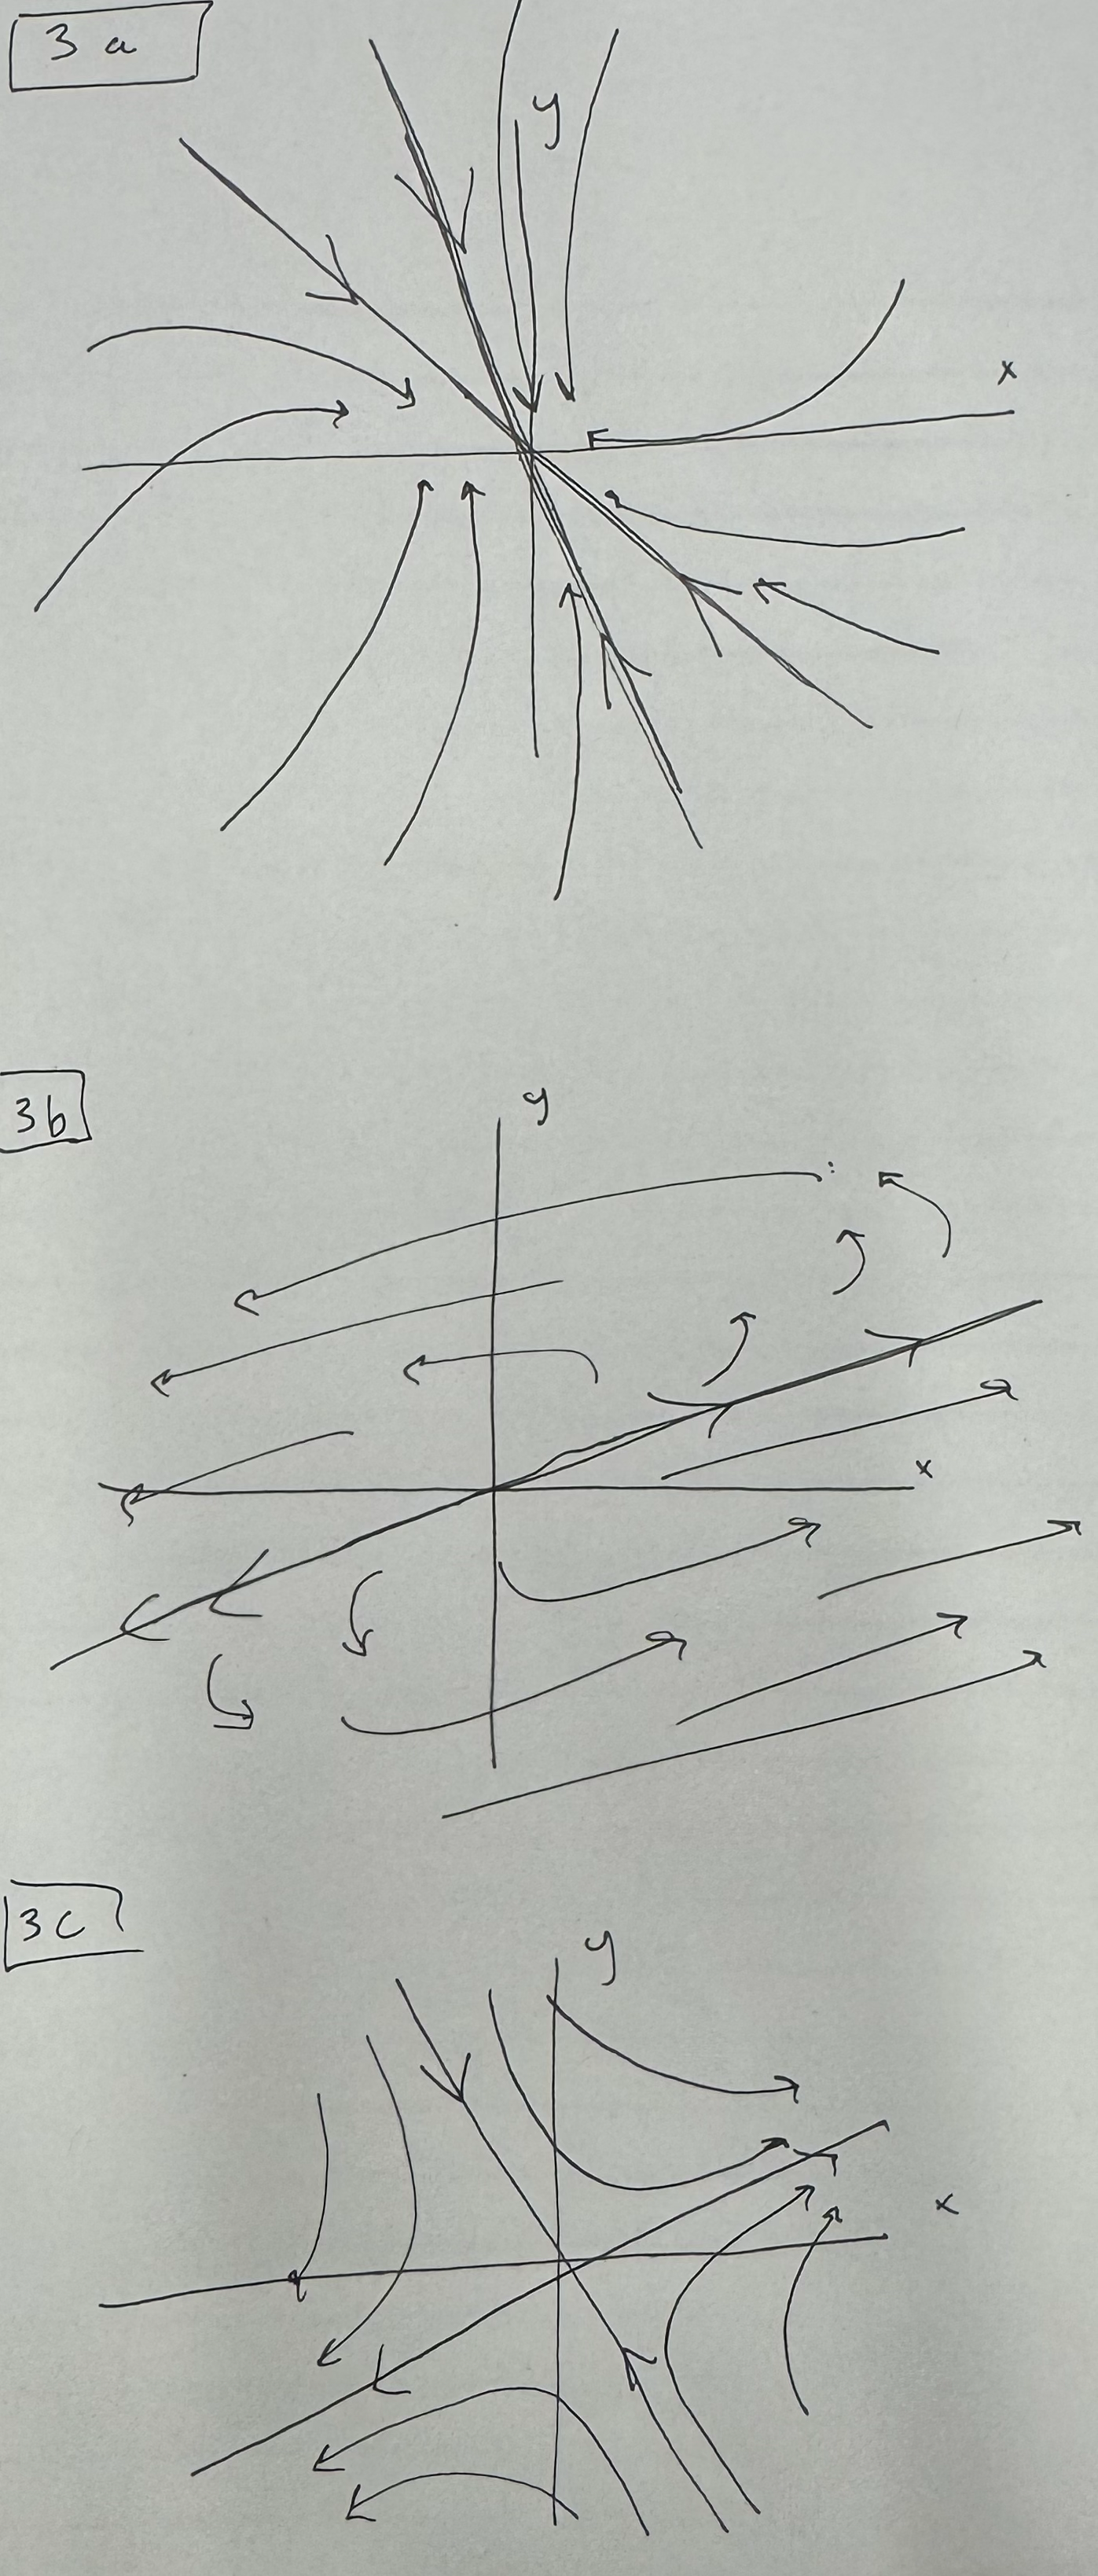
\includegraphics[height=.8\textwidth]{3_a_c.png}
 	\caption{In this figure we describe the qualitative behavior of the two dimensional phase portraits.}
	\label{fig:f4}
\end{figure}
\qed \\

\item $\dot x = 3x - 4y, \quad \dot y = x - y$ \\
\textit{Solution:} \\
We can put this in the form of a 2 dimensional first order system as follows
\begin{align*}
\begin{bmatrix}
x \\ y
\end{bmatrix}^\prime
&= \begin{bmatrix}
3 & -4 \\
1 & -1
\end{bmatrix} \begin{bmatrix}
x \\ y
\end{bmatrix}
\end{align*}
We need to calculate eigenvalues using the characteristic equation which is 
$$(3 - \lambda)(-1 -\lambda) + 4.$$
Then
\begin{align*}
-3 + \lambda -3\lambda + \lambda^2 + 4 &= 0 \\
\lambda^2 -2\lambda + 1 &= 0 \\
(\lambda - 1)^2 &= 0.
\end{align*}
Then we have $\lambda = 1$ with algebraic multiplicity of 2.
Now for the eigenvectors!
\begin{align*}
\begin{bmatrix}
2 & -4 \\
1 & -2
\end{bmatrix} \begin{bmatrix}
x \\ y
\end{bmatrix} = \bm 0.
\end{align*}
Therefore we have $2x -4y = 0$ then $x = 2y$ and $y = y$ therefore the eigenvector is
\begin{align*}
\begin{bmatrix} 2 \\ 1 \end{bmatrix}.
\end{align*} 
Now we can draw the qualitative phase portrait, see Figure \ref{fig:f4} \\

\item $\ddot x + 2\dot x - x = 0$ \\
\textit{Solution:} \\
We can put this second order system in the form of a 2 dimensional first order system as follows.
Set $x_1 = x$ and $x_2 = \dot x$
\begin{align*}
\begin{bmatrix}
x_1 \\ x_2
\end{bmatrix}^\prime
&= \begin{bmatrix}
0 & 1 \\
1 & -2
\end{bmatrix} \begin{bmatrix}
x_1 \\ x_2
\end{bmatrix}.
\end{align*}
Therefore,
\begin{align*}
-\lambda(-2 -\lambda) - 1 &= 0 \\
2\lambda + \lambda^2 - 1 &= 0.
\end{align*}
Then we have
$$
\lambda = \frac{-2 \pm \sqrt{4 +4}} 2 = -1 \pm \sqrt 2.
$$
The eigenvectors are
\begin{align*}
\begin{bmatrix} 1 + \sqrt 2 \\ 1 \end{bmatrix} \quad {\rm and} \quad
\begin{bmatrix} 1 - \sqrt 2 \\ 1 \end{bmatrix}.
\end{align*} 
We have an unstable attractor or a saddle node fixed point since the eigenvalues are both real and one is positive and the other is negative.
See Figure \ref{fig:f4} for the actual phase portrait.

\end{enumerate}

\newpage

\item There is a lot of context and build up to this problem in the assignment pdf which I will not transcribe here.
The important details will be included in their respective parts. \\

\begin{enumerate}

\item Rewrite the second-order differential equation
$$L \ddot I + \dot I R + \frac I C = 0$$
as a 2-D linear dynamical system. \\
\textit{Solution:} \\
If we let $I_1 = I$ and $I_2 = \dot I$ then we have
\begin{align*}
\begin{bmatrix}
I_1 \\ I_2
\end{bmatrix}^\prime
&= \begin{bmatrix}
0 & 1 \\
-\frac 1 {LC} & -\frac R L
\end{bmatrix} \begin{bmatrix}
I_1 \\ I_2
\end{bmatrix}
\end{align*}
\qed \\

\item Show that the origin is asymptotically stable if $R > 0$ and neutrally stable if $R = 0$. \\
\textit{Solution:} \\
In order to classify it in these scenarios we want to calculate the eigenvalues of the matrix representing our DS.
We first need to calculate the characteristic equation as follows
\begin{align*}
-\lambda \left(- \frac R L - \lambda \right) + \frac 1 {LC} &= 0 \\
\lambda^2 + \lambda \frac R L + \frac 1 {LC} &= 0.
\end{align*}
This gives us
\begin{equation}
\lambda = \frac {-R/L \pm \sqrt{R^2/L^2 - 4/(LC)} }{2}.
\label{eq:eq2}
\end{equation}
Now if $R > 0$, then the origin is asymptotically stable since the real part of the eigenvalues will be negative.
However, if $R = 0$ then the real part of the eigenvalues is $0$ or rather the eigenvalues are purely imaginary, then the origin will be neutrally stable. \\
\qed \\

\item Classify the fixed point at the origin depending on whether $R^2C - 4L$ is positive, negative, or zero. \\
\textit{Solution:} \\
Referring back to equation (\ref{eq:eq2}) we can see that the value of interest here is within a scalar of the discriminant which determines whether or not there is any imaginary component to the eigenvalues.
See the following minor rewriting of equation (\ref{eq:eq2})
\begin{align*}
\lambda &= \frac {-R/L \pm \sqrt{R^2/L^2 - 4/(LC)} }{2} \\
\lambda &= \frac {-R/L \pm \sqrt{(R^2 - 4L/C)/L^2} }{2} \\
\lambda &= \frac {-R/L \pm \sqrt{(R^2C - 4L)/(L^2C)} }{2}.
\end{align*}
Since we are given in the problem statement that $C > 0$ and $L > 0$, then $L^2C > 0$.
Therefore, the sign of the discriminant and therefore it's real or imaginaryness is determined purely by the value of $R^2C - 4L$.
Now if $R^2C - 4L > 0$ then the eigenvalues will be entirely real but their sign depends on the sign of $R$.
If $R > 0$ then we have negative real valued eigenvalues which implies that the system is a sink/attractor.
Now if $R^2C - 4L = 0$ then the eigenvalues will be entirely real but their sign depends on the sign of $R$ again.
If $R > 0$ then we have negative real valued eigenvalues which implies that the system is a sink/attractor.
Now if $R^2C - 4L < 0$ then the eigenvalues will have an imaginary component.
This means there will be some oscillatory effects in the solutions but yet again still depends on the value of $R$.
It could be neutrally stable if $R = 0$ it could also be either a sink or a source depending on the sign of $R$. \\
\qed \\

\end{enumerate}

\newpage

\item We will be modeling the feelings of affection between $R$ and $J$, where
\begin{align*}
R(t) &= \text{ $R$’s feelings for $J$ at time $t$, } \\
J(t) &= \text{ $J$’s feelings for $R$ at time $t$. }
\end{align*}
When $R$ or $J$ is positive, the feeling is a positive feeling (endearment).
When $R$ or $J$ is negative, the feeling is a negative feeling (animus).
Consider the following dynamical system governing the relationship between $R$ and $J$,
\begin{align*}
\dot R &= aR + J \\
\dot J &= -R -a J
\end{align*}
where $a > 0$ is a constant. \\

\begin{enumerate}

\item (Not graded) Try to explain how $R$ and $J$ respond to their own feelings and to each other’s feelings.
What role does the parameter $a$ play?
This should be a text-response, not calculations. \\
\textit{Solution:} \\
Romeo ($R$) amplifies his own feelings and Juliet's ($J$) as well.
So his feelings change positively if his own and Juliet's are positive and the opposite holds true as well if their feelings are negative.
On the other hand Juliet's feelings change in the opposite direction of the current feelings, so if she feels positively and or Romeo feels positively then her feelings will decrease.
\\
\qed

\item Do the following for $a > 1$ and $ a < 1$ \\

\begin{enumerate}

\item Determine whether the origin is asymptotically stable, neutrally stable, unstable and attracting, or unstable and not attracting.
Also classify the origin as a saddle point, node, center, or spiral.
If the origin is a saddle point, identify (either by highlighting or explaining with words/formulae) the stable and unstable manifolds. \\
\textit{Solution:} \\
First turning this into a system of first orders in matrix form we have
\begin{align*}
\begin{bmatrix}
R \\ J
\end{bmatrix}^\prime
&= \begin{bmatrix}
a & 1 \\
-1 & -a
\end{bmatrix} \begin{bmatrix}
R \\ J
\end{bmatrix}.
\end{align*}
Then the characteristic equation to calculate eigenvalues is the following
\begin{align*}
(a - \lambda)(-a - \lambda) + 1 &= 0 \\
-a^2 + \lambda^2 + 1 &= 0 \\
\lambda^2 - a^2 + 1 &= 0 \\
\lambda^2 &= a^2 - 1 \\
\lambda &= \sqrt{a^2 - 1}.
\end{align*}
Now if $a < 1$ then the eigenvalue, $\lambda$, is purely imaginary and thus the origin is a neutrally stable fixed point also known as a center.
However, if $a > 1$ then the eigenvalues are purely real and of opposite sign.
Therefore the origin is a saddle node and is unstable and attracting. \\
\qed \\

\item Verify what you found in part (i) with a plot of the phase portrait (using pplane).
You may choose a particular value of $a$ for plotting.
Interpret the long-time behavior of the system in terms of $R$ and $J$’s relationship. \\
\textit{Solution:} \\
In the scenario where $a > 1$ then the couple will attract one another feeling greater and greater affection until they reach a maximum and shoot off to infinity away from one another and then they will not like one another ever again.
Interestingly enough in the $a < 1$ case they will always orbit around affection for each other but will never settle in to a single particular value of affection just oscillating or orbiting in a particular tier. \\
\qed \\

\end{enumerate}

\item Summarize and interpret what you found in part (b).
How does the size of $a$ play out in $J$ and $R$’s relationship? \\
\textit{Solution:} \\
I would say that the size of $a$ would result in how rapidly they achiev the end state (at least for $a > 1$).
When $a < 1$ then they just orbit around the same state's all the time. \\
\qed \\

\end{enumerate}

\end{enumerate}

\end{document}

%%% Local Variables:
%%% mode: latex
%%% TeX-master: t
%%% End:
